\Chapter{Results}
\label{chap:results}

\section{Evaluation Setup}
\Todo{Briefly restate dataset and metrics. Point to Methods for details; specify commit hash and config used for final runs.}

\section{Overall Transplantation Performance}
\Todo{Report counts: number of targets, donors found, ligands considered, successful transplants. Include a summary table.}

\section{Quality Indicators}
\Todo{Present distributions of RMSD, clash scores, and confidence indicators. Add figure placeholders.}
% \begin{figure}[t]
%   \centering
%   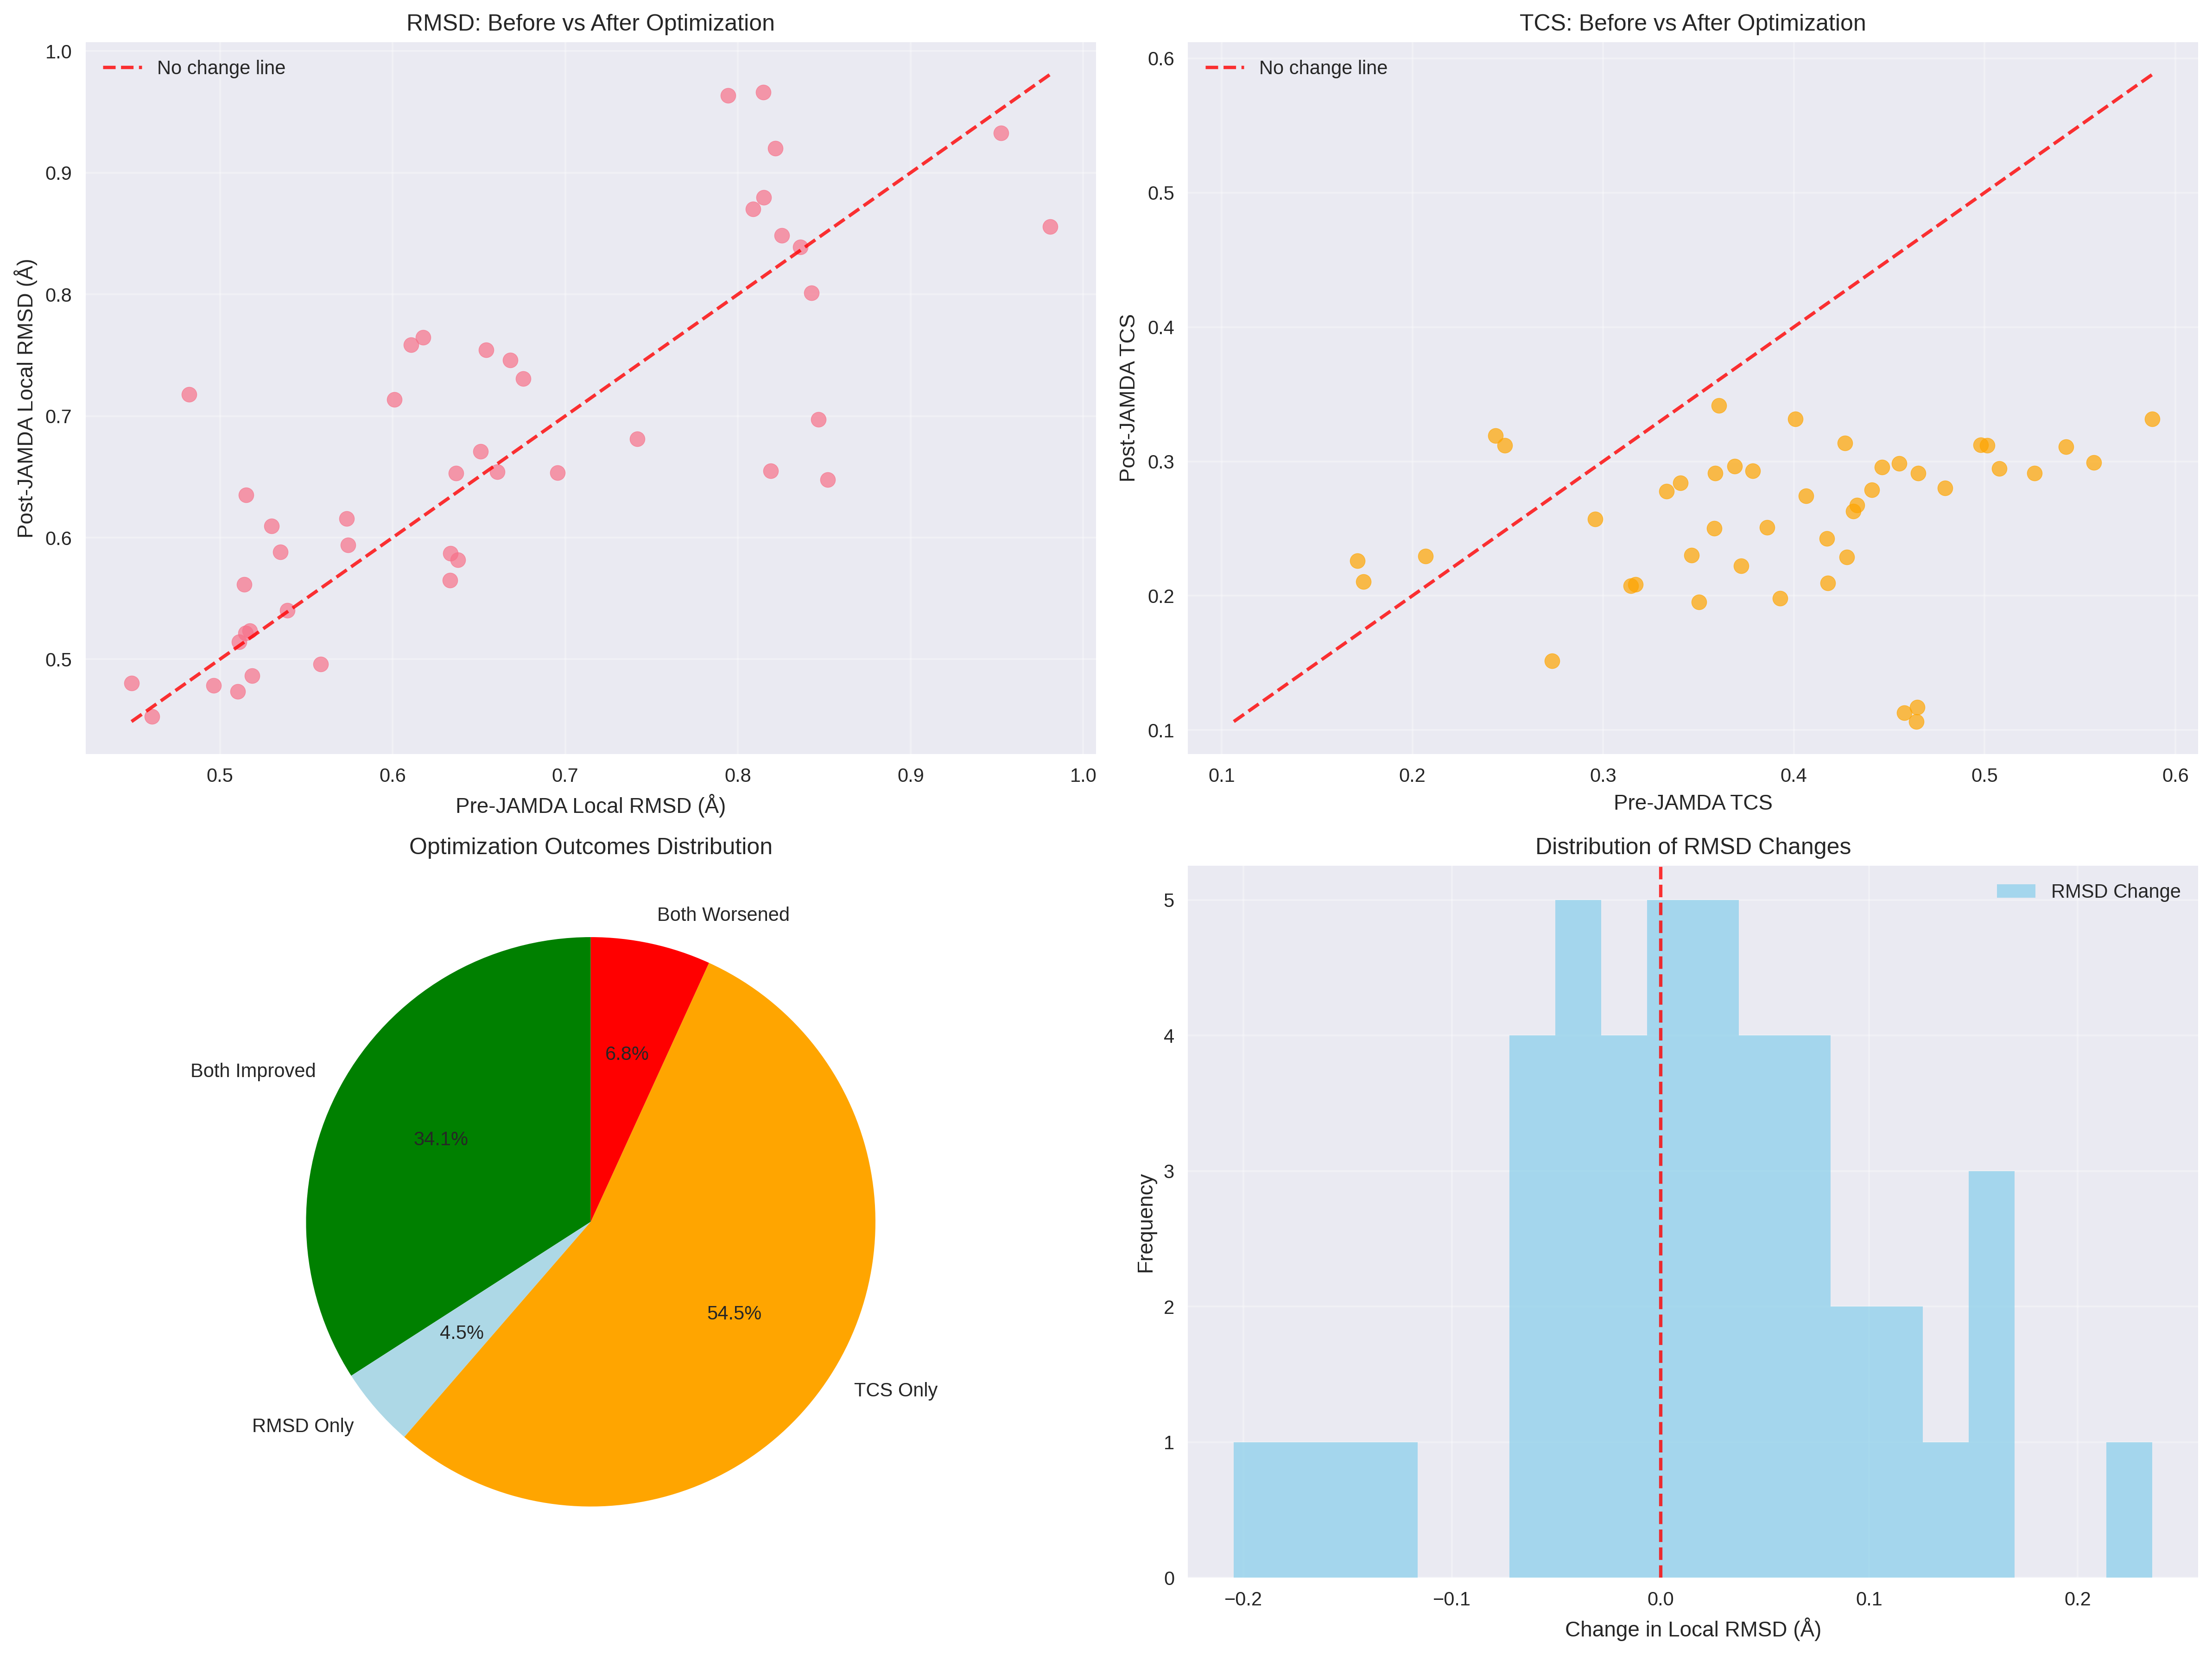
\includegraphics[width=0.9\linewidth]{figures/optimization_effectiveness.png}
%   \caption{Placeholder: quality indicator distribution. Replace with final plot export.}
%   \label{fig:quality_indicators}
% \end{figure}

\section{Alignment Quality Analysis}
\Todo{Insert analysis and figure from \texttt{scripts/evaluation\_visualisations.py}. Explain trends and outliers.}
% Example reference to existing asset if exported to thesis/figures
% 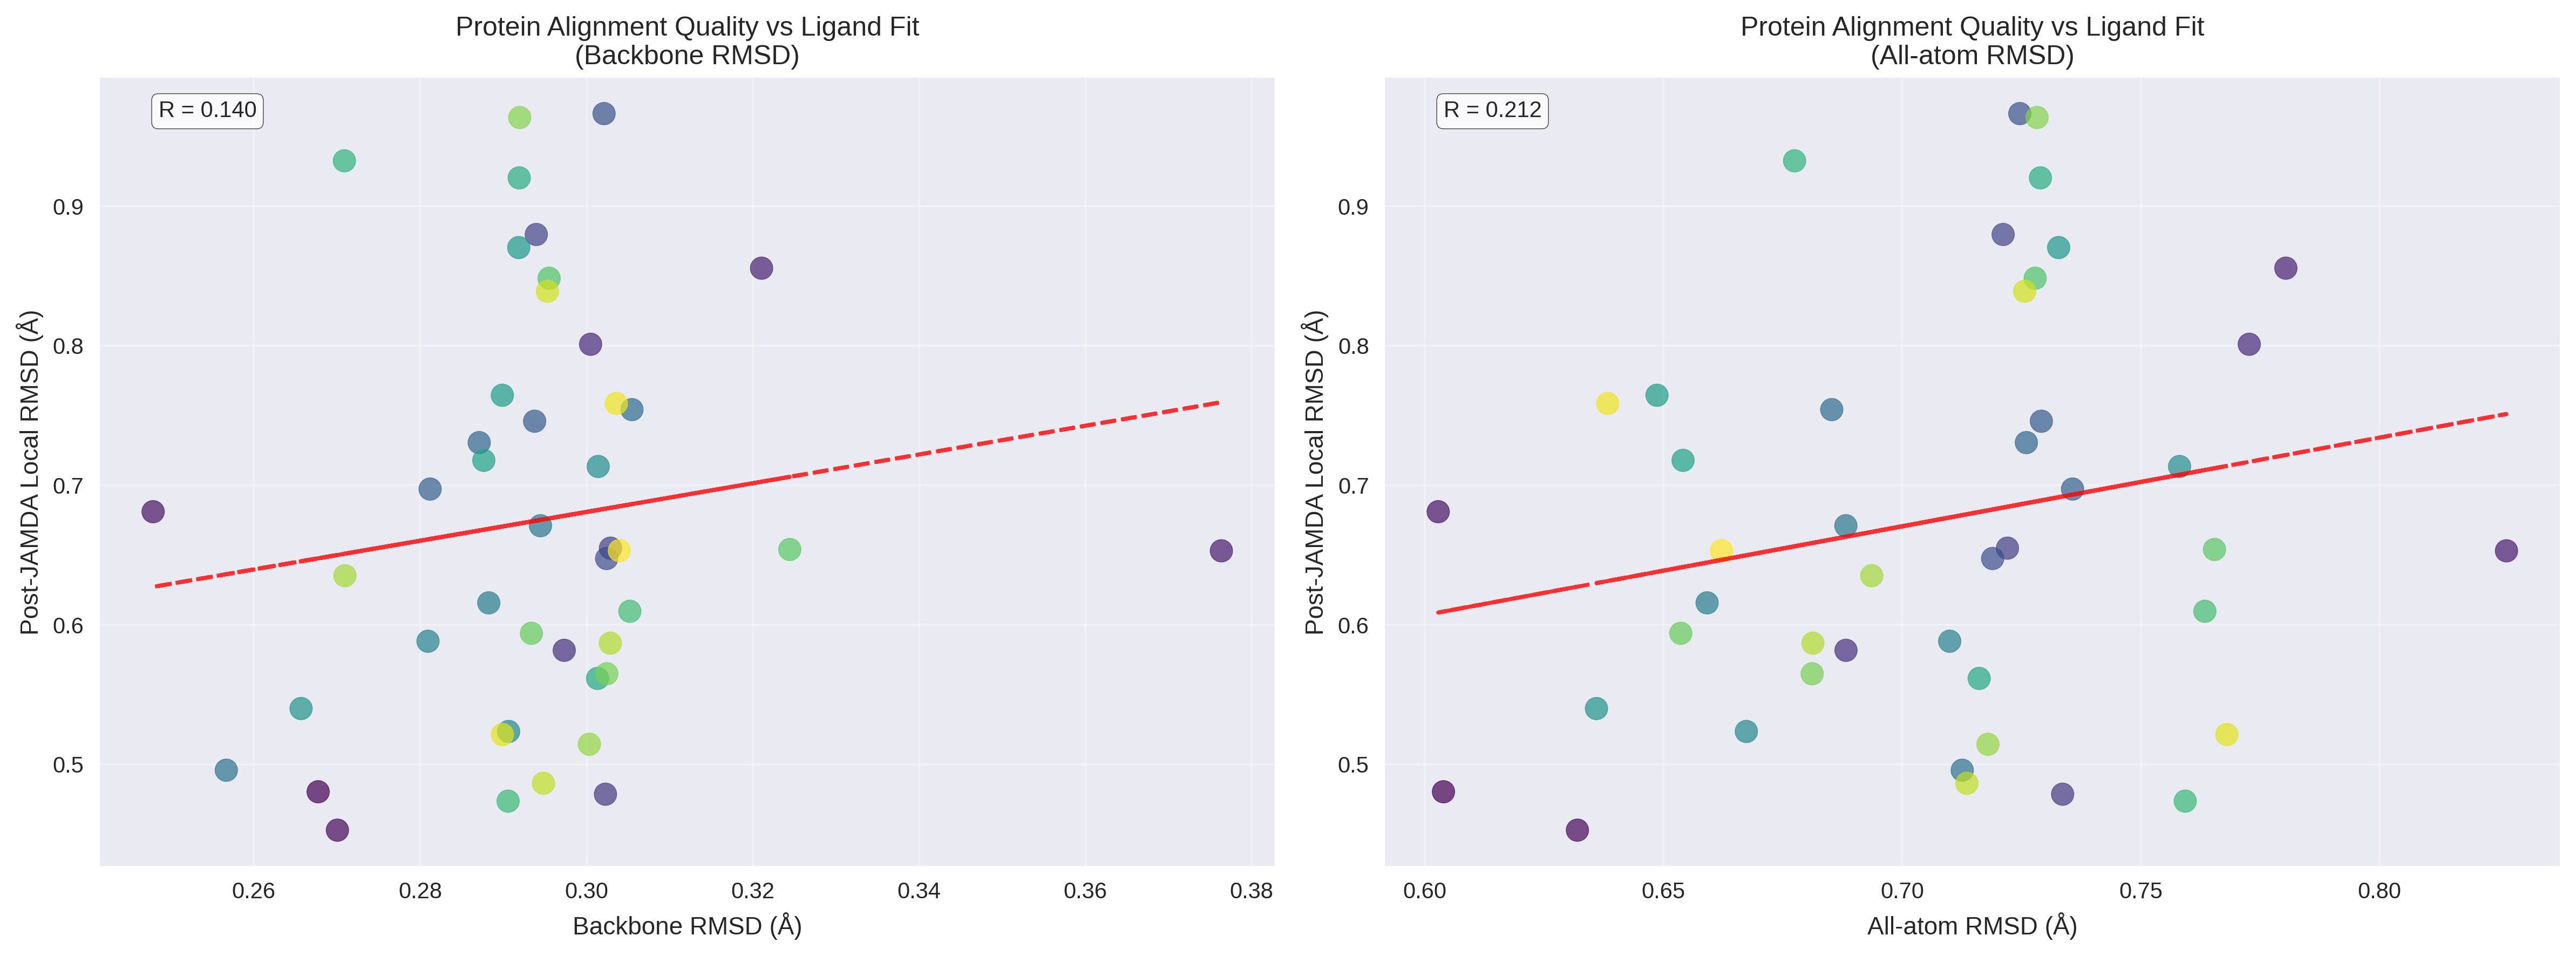
\includegraphics[width=0.9\linewidth]{figures/alignment_quality_analysis.png}

\section{Optimization and Filtering Effects}
\Todo{Show before/after metrics; explain trade-offs. Include relevant figures (\texttt{optimization\_*}).}

\section{Case Studies}
\Todo{Pick 2–3 representative proteins; show visualizations (ligand placement), discuss plausibility and caveats.}

\section{Failure Modes}
\Todo{Describe common errors (misaligned donors, steric clashes, metal coordination errors) with examples and how filters mitigate them.}

\section{Ablations (optional)}
\Todo{If available, compare alternative alignment thresholds or scoring components. Summarize in a small table.}
